% Page 3: request flow and contracts.
\subsection{HTTP 请求处理与接口契约}
页面查询和内容提交的处理流程见图\ref{fig:design-http-flow}。服务端先识别请求访问的资源和操作类型。需要登录的请求先验证身份；如果资源属于他人或某个会话，还需校验当前用户对该资源的访问权限。

\begin{figure}[H]
\centering
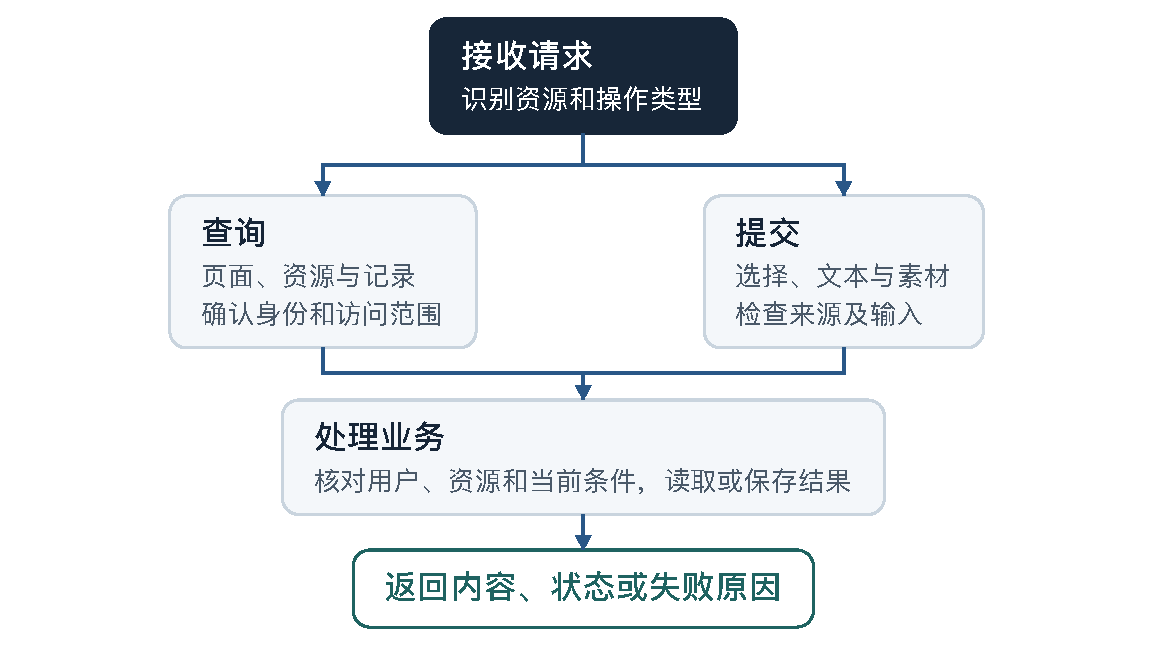
\includegraphics[width=.88\linewidth]{assets/design/http-flow.pdf}
\caption{请求接收、业务检查与结果返回流程}\label{fig:design-http-flow}
\end{figure}

查询用于读取当前记录。提交接口接收同源 JSON 请求。普通请求体上限为 64\,000 字节，媒体上传放宽至 4\,200\,000 字节。通过来源、格式和输入校验后，再判断业务条件。比如读写聊天消息时，服务端根据会话编号找到记录，确认当前用户是会话参与者后才继续。

对于未登录的用户，页面引导其登录。输入校验失败时，页面提示修改。如果业务条件已经变化，接口返回当前结果，页面据此提示用户下一步能做什么。

\begin{table}[H]
\centering\small\linespread{1.15}\selectfont
\caption{代表业务操作及处理结果}\label{tab:design-api-summary}
\begin{tabularx}{\linewidth}{@{}p{.34\linewidth}X@{}}
\toprule 业务操作 & 用户选择与核心结果 \\ \midrule
进入个人页面 & 获取本人资料、互动和形象摘要，展示已有记录与辅助能力的可用状态 \\
发现相遇对象 & 由服务端选择候选；已有待决定卡片时继续展示该卡，等待收藏或跳过 \\
处理收到的纸条 & 收件人选择接受并回信或拒绝；接受后建立会话，拒绝则结束本次邀请 \\
申请情绪立绘 & 用户选择情绪并同意生成；服务端返回任务状态，完成后由用户查看预览并确认保存 \\
\bottomrule
\end{tabularx}
\end{table}

页面分别显示完成、等待和失败。接口摘要见附录表\ref{tab:compact-api}。

\clearpage
